\section{config\_\-params.h File Reference}
\label{config__params_8h}\index{config\_\-params.h@{config\_\-params.h}}
{\tt \#include \char`\"{}simIrisComponentHeader.h\char`\"{}}\par
{\tt \#include \char`\"{}genericData.h\char`\"{}}\par
{\tt \#include \char`\"{}mc\_\-constants.h\char`\"{}}\par


Include dependency graph for config\_\-params.h:\nopagebreak
\begin{figure}[H]
\begin{center}
\leavevmode
\includegraphics[width=298pt]{config__params_8h__incl}
\end{center}
\end{figure}


This graph shows which files directly or indirectly include this file:\nopagebreak
\begin{figure}[H]
\begin{center}
\leavevmode
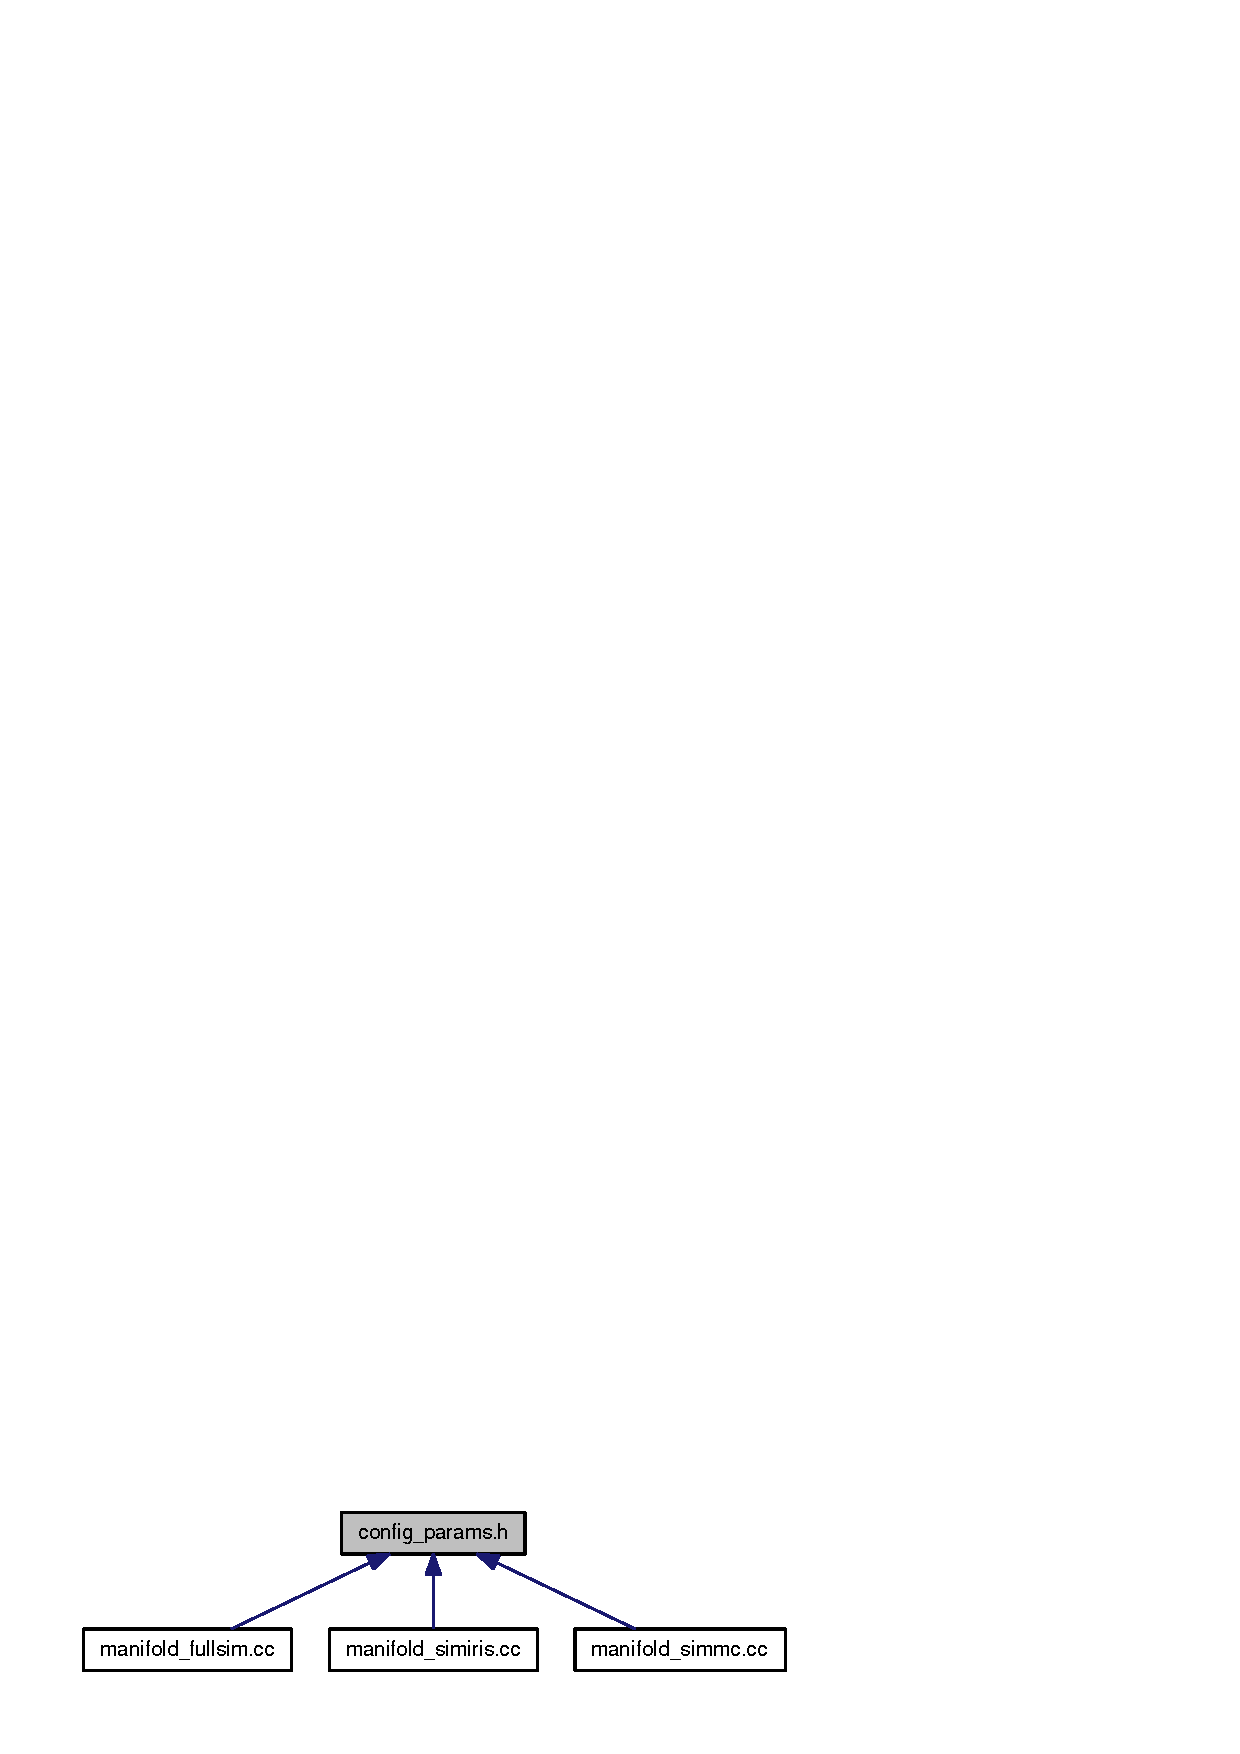
\includegraphics[width=190pt]{config__params_8h__dep__incl}
\end{center}
\end{figure}
\subsection*{Functions}
\begin{CompactItemize}
\item 
void {\bf init\_\-dram\_\-timing\_\-parameters} (void)
\end{CompactItemize}
\subsection*{Variables}
\begin{CompactItemize}
\item 
{\bf uint} {\bf no\_\-nodes} = 0
\item 
{\bf uint} {\bf no\_\-mcs} = 0
\item 
{\bf uint} {\bf do\_\-two\_\-stage\_\-router} = 0
\item 
{\bf uint} {\bf max\_\-phy\_\-link\_\-bits} = 128
\item 
{\bf uint} {\bf links} = 0
\item 
{\bf ullint} {\bf max\_\-sim\_\-time} = 1000000
\item 
{\bf ROUTING\_\-SCHEME} {\bf rc\_\-method} = XY
\item 
{\bf SW\_\-ARBITRATION} {\bf sw\_\-arbitration} = ROUND\_\-ROBIN
\item 
{\bf ROUTER\_\-MODEL} {\bf router\_\-model} = PHYSICAL\_\-3STAGE
\item 
{\bf MC\_\-MODEL} {\bf mc\_\-model} = GENERIC\_\-MC
\item 
{\bf message\_\-class} {\bf priority\_\-msg\_\-type} = PRIORITY\_\-REQ
\item 
{\bf uint} {\bf print\_\-setup} = 0
\item 
{\bf uint} {\bf grid\_\-size} = 0
\item 
const bool {\bf multiple\_\-flit\_\-in\_\-buf} = true
\item 
vector$<$ {\bf uint} $>$ {\bf mc\_\-positions}
\item 
vector$<$ string $>$ {\bf traces}
\item 
{\bf uint} {\bf vcs} = 0
\item 
{\bf uint} {\bf ports} = 0
\item 
{\bf uint} {\bf buffer\_\-size} = 0
\item 
{\bf uint} {\bf credits} = 0
\item 
string {\bf trace\_\-name}
\item 
string {\bf output\_\-path}
\item 
string {\bf msg\_\-type\_\-string}
\item 
string {\bf routing\_\-scheme}
\item 
string {\bf sw\_\-arbitration\_\-scheme}
\item 
string {\bf addr\_\-map\_\-scheme\_\-string}
\item 
string {\bf mc\_\-scheduling\_\-algorithm\_\-string}
\item 
string {\bf dram\_\-page\_\-policy\_\-string}
\item 
{\bf uint} {\bf THREAD\_\-BITS\_\-POSITION} = 25
\item 
{\bf uint} {\bf MC\_\-ADDR\_\-BITS} = 12
\item 
{\bf uint} {\bf BANK\_\-BITS} = 13
\item 
{\bf DRAM\_\-CONFIG} {\bf dram\_\-config\_\-string} = DDR3\_\-1600\_\-10
\item 
{\bf DRAM\_\-PAGE\_\-POLICY} {\bf dram\_\-page\_\-policy} = OPEN\_\-PAGE\_\-POLICY
\item 
{\bf MC\_\-SCHEDULLING\_\-ALGO} {\bf mc\_\-scheduling\_\-algorithm} = FR\_\-FCFS
\item 
{\bf ADDR\_\-MAP\_\-SCHEME} {\bf addr\_\-map\_\-scheme} = PAGE\_\-INTERLEAVING
\item 
{\bf uint} {\bf NO\_\-OF\_\-THREADS} = 2
\item 
{\bf uint} {\bf MAX\_\-BUFFER\_\-SIZE} = 8
\item 
{\bf uint} {\bf MAX\_\-CMD\_\-BUFFER\_\-SIZE} = 16
\item 
{\bf uint} {\bf RESPONSE\_\-BUFFER\_\-SIZE} = 56$\ast$8
\item 
{\bf uint} {\bf NO\_\-OF\_\-RANKS} = 1
\item 
{\bf uint} {\bf NO\_\-OF\_\-BANKS} = 8
\item 
{\bf uint} {\bf NO\_\-OF\_\-ROWS} = 8192
\item 
{\bf uint} {\bf NO\_\-OF\_\-COLUMNS} = 128
\item 
{\bf uint} {\bf COLUMN\_\-SIZE} = 64
\item 
{\bf uint} {\bf NETWORK\_\-ADDRESS\_\-BITS} = 48
\item 
{\bf uint} {\bf NETWORK\_\-THREADID\_\-BITS} = 6
\item 
{\bf uint} {\bf NETWORK\_\-COMMAND\_\-BITS} = 3
\item 
{\bf uint} {\bf MSHR\_\-SIZE} = 8
\item 
float {\bf CORE\_\-SPEED} = 3000
\item 
float {\bf CYCLE\_\-2\_\-NS} = ({\bf CORE\_\-SPEED}$\ast$1.0 / 1000)
\item 
{\bf uint} {\bf DDR\_\-BUS\_\-WIDTH}
\item 
float {\bf BUS\_\-SPEED}
\item 
float {\bf MEM\_\-SPEED}
\item 
float {\bf MEM\_\-CYCLE}
\item 
float {\bf BUS\_\-CYCLE}
\item 
float {\bf tREFI}
\item 
float {\bf tRFC}
\item 
float {\bf tRC}
\item 
float {\bf tRAS}
\item 
{\bf uint} {\bf t\_\-CMD}
\item 
{\bf uint} {\bf t\_\-RCD}
\item 
{\bf uint} {\bf t\_\-RRD}
\item 
{\bf uint} {\bf t\_\-RAS}
\item 
{\bf uint} {\bf t\_\-CAS}
\item 
{\bf uint} {\bf t\_\-RTRS}
\item 
{\bf uint} {\bf t\_\-OST}
\item 
{\bf uint} {\bf t\_\-WR}
\item 
{\bf uint} {\bf t\_\-WTR}
\item 
{\bf uint} {\bf t\_\-RP}
\item 
{\bf uint} {\bf t\_\-CCD}
\item 
{\bf uint} {\bf t\_\-AL}
\item 
{\bf uint} {\bf t\_\-CWD}
\item 
{\bf uint} {\bf t\_\-RC}
\item 
{\bf uint} {\bf t\_\-RTP}
\item 
{\bf uint} {\bf t\_\-RFC}
\end{CompactItemize}


\subsection{Function Documentation}
\index{config\_\-params.h@{config\_\-params.h}!init\_\-dram\_\-timing\_\-parameters@{init\_\-dram\_\-timing\_\-parameters}}
\index{init\_\-dram\_\-timing\_\-parameters@{init\_\-dram\_\-timing\_\-parameters}!config_params.h@{config\_\-params.h}}
\subsubsection[{init\_\-dram\_\-timing\_\-parameters}]{\setlength{\rightskip}{0pt plus 5cm}void init\_\-dram\_\-timing\_\-parameters (void)}\label{config__params_8h_a91b414eca2957d22f6a86c695a803c6}




Definition at line 118 of file config\_\-params.h.

References BUS\_\-CYCLE, BUS\_\-SPEED, CORE\_\-SPEED, CYCLE\_\-2\_\-NS, DDR2\_\-533\_\-4, DDR2\_\-667\_\-4, DDR3\_\-1333\_\-6, DDR3\_\-1333\_\-9, DDR3\_\-1600\_\-10, DDR\_\-BUS\_\-WIDTH, dram\_\-config\_\-string, MEM\_\-CYCLE, MEM\_\-SPEED, t\_\-AL, t\_\-CAS, t\_\-CCD, t\_\-CMD, t\_\-CWD, t\_\-OST, t\_\-RAS, t\_\-RC, t\_\-RCD, t\_\-RFC, t\_\-RP, t\_\-RRD, t\_\-RTP, t\_\-RTRS, t\_\-WR, t\_\-WTR, tRAS, tRC, tREFI, and tRFC.

Referenced by main().

Here is the caller graph for this function:\nopagebreak
\begin{figure}[H]
\begin{center}
\leavevmode
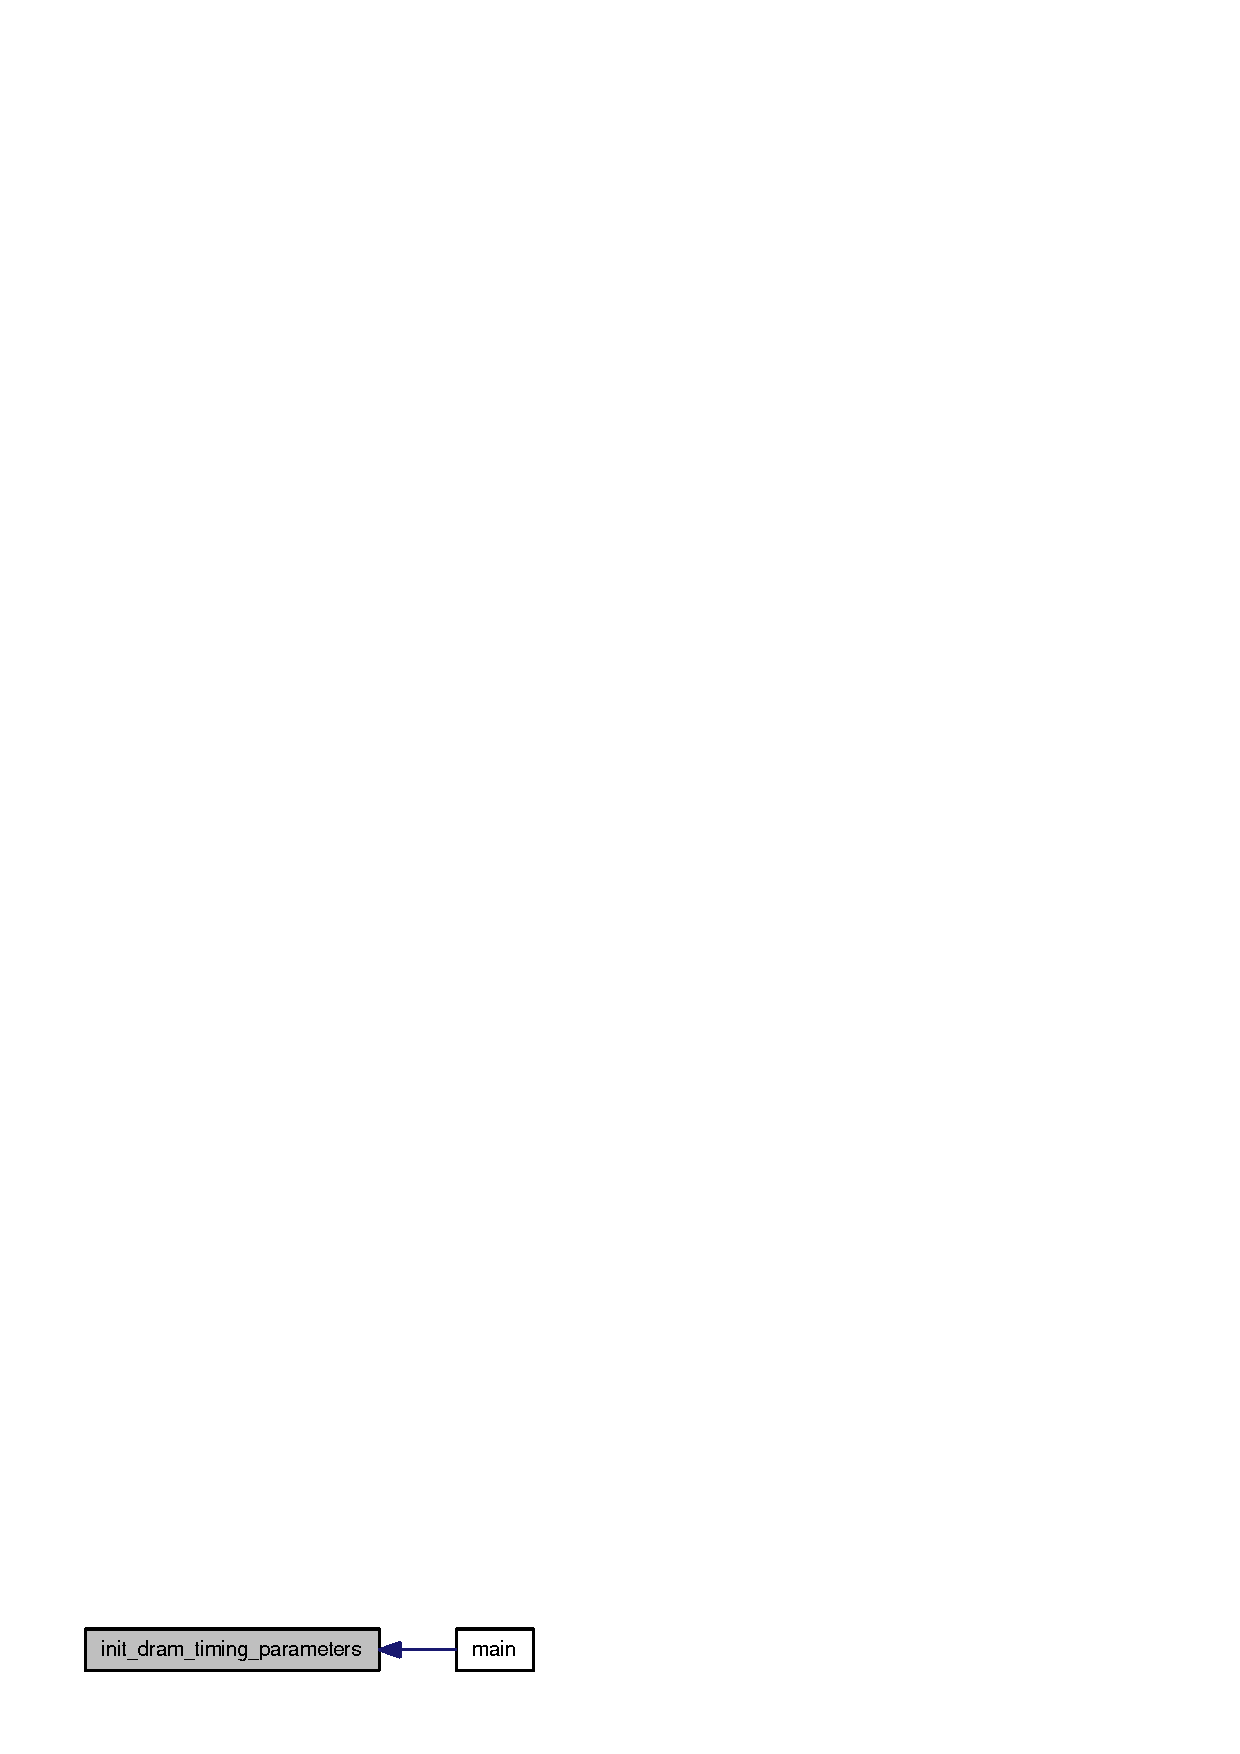
\includegraphics[width=130pt]{config__params_8h_a91b414eca2957d22f6a86c695a803c6_icgraph}
\end{center}
\end{figure}


\subsection{Variable Documentation}
\index{config\_\-params.h@{config\_\-params.h}!addr\_\-map\_\-scheme@{addr\_\-map\_\-scheme}}
\index{addr\_\-map\_\-scheme@{addr\_\-map\_\-scheme}!config_params.h@{config\_\-params.h}}
\subsubsection[{addr\_\-map\_\-scheme}]{\setlength{\rightskip}{0pt plus 5cm}{\bf ADDR\_\-MAP\_\-SCHEME} {\bf addr\_\-map\_\-scheme} = PAGE\_\-INTERLEAVING}\label{config__params_8h_d1a6650288eeca57ccc26007fe8b2ebe}




Definition at line 61 of file config\_\-params.h.\index{config\_\-params.h@{config\_\-params.h}!addr\_\-map\_\-scheme\_\-string@{addr\_\-map\_\-scheme\_\-string}}
\index{addr\_\-map\_\-scheme\_\-string@{addr\_\-map\_\-scheme\_\-string}!config_params.h@{config\_\-params.h}}
\subsubsection[{addr\_\-map\_\-scheme\_\-string}]{\setlength{\rightskip}{0pt plus 5cm}string {\bf addr\_\-map\_\-scheme\_\-string}}\label{config__params_8h_c4c6117e0110c4a18bdd2b1360cc36e5}




Definition at line 51 of file config\_\-params.h.

Referenced by main().\index{config\_\-params.h@{config\_\-params.h}!BANK\_\-BITS@{BANK\_\-BITS}}
\index{BANK\_\-BITS@{BANK\_\-BITS}!config_params.h@{config\_\-params.h}}
\subsubsection[{BANK\_\-BITS}]{\setlength{\rightskip}{0pt plus 5cm}{\bf uint} {\bf BANK\_\-BITS} = 13}\label{config__params_8h_40e7d425b08789ca96de0a1bc3af2803}




Definition at line 54 of file config\_\-params.h.

Referenced by dump\_\-configuration(), iris\_\-process\_\-options(), main(), and AddrMap::map\_\-addr().\index{config\_\-params.h@{config\_\-params.h}!buffer\_\-size@{buffer\_\-size}}
\index{buffer\_\-size@{buffer\_\-size}!config_params.h@{config\_\-params.h}}
\subsubsection[{buffer\_\-size}]{\setlength{\rightskip}{0pt plus 5cm}{\bf uint} {\bf buffer\_\-size} = 0}\label{config__params_8h_c9ed472f13d0eb7f926e286e05bfbcc7}




Definition at line 48 of file config\_\-params.h.

Referenced by dump\_\-configuration(), iris\_\-init(), iris\_\-process\_\-options(), and main().\index{config\_\-params.h@{config\_\-params.h}!BUS\_\-CYCLE@{BUS\_\-CYCLE}}
\index{BUS\_\-CYCLE@{BUS\_\-CYCLE}!config_params.h@{config\_\-params.h}}
\subsubsection[{BUS\_\-CYCLE}]{\setlength{\rightskip}{0pt plus 5cm}float {\bf BUS\_\-CYCLE}}\label{config__params_8h_6905232b437897dbbc50631f4592275e}




Definition at line 95 of file config\_\-params.h.\index{config\_\-params.h@{config\_\-params.h}!BUS\_\-SPEED@{BUS\_\-SPEED}}
\index{BUS\_\-SPEED@{BUS\_\-SPEED}!config_params.h@{config\_\-params.h}}
\subsubsection[{BUS\_\-SPEED}]{\setlength{\rightskip}{0pt plus 5cm}float {\bf BUS\_\-SPEED}}\label{config__params_8h_97f1347e6a89939a723b3cdd452c76cb}




Definition at line 92 of file config\_\-params.h.\index{config\_\-params.h@{config\_\-params.h}!COLUMN\_\-SIZE@{COLUMN\_\-SIZE}}
\index{COLUMN\_\-SIZE@{COLUMN\_\-SIZE}!config_params.h@{config\_\-params.h}}
\subsubsection[{COLUMN\_\-SIZE}]{\setlength{\rightskip}{0pt plus 5cm}{\bf uint} {\bf COLUMN\_\-SIZE} = 64}\label{config__params_8h_f0596ae8862443e137eb225092bffad6}




Definition at line 76 of file config\_\-params.h.\index{config\_\-params.h@{config\_\-params.h}!CORE\_\-SPEED@{CORE\_\-SPEED}}
\index{CORE\_\-SPEED@{CORE\_\-SPEED}!config_params.h@{config\_\-params.h}}
\subsubsection[{CORE\_\-SPEED}]{\setlength{\rightskip}{0pt plus 5cm}float {\bf CORE\_\-SPEED} = 3000}\label{config__params_8h_caed83499d078ca4534df759dc75445c}




Definition at line 88 of file config\_\-params.h.\index{config\_\-params.h@{config\_\-params.h}!credits@{credits}}
\index{credits@{credits}!config_params.h@{config\_\-params.h}}
\subsubsection[{credits}]{\setlength{\rightskip}{0pt plus 5cm}{\bf uint} {\bf credits} = 0}\label{config__params_8h_a0f16f2b9c6bb8d38139a2b9f520d184}




Definition at line 48 of file config\_\-params.h.

Referenced by dump\_\-configuration(), iris\_\-init(), iris\_\-process\_\-options(), and main().\index{config\_\-params.h@{config\_\-params.h}!CYCLE\_\-2\_\-NS@{CYCLE\_\-2\_\-NS}}
\index{CYCLE\_\-2\_\-NS@{CYCLE\_\-2\_\-NS}!config_params.h@{config\_\-params.h}}
\subsubsection[{CYCLE\_\-2\_\-NS}]{\setlength{\rightskip}{0pt plus 5cm}float {\bf CYCLE\_\-2\_\-NS} = ({\bf CORE\_\-SPEED}$\ast$1.0 / 1000)}\label{config__params_8h_95a920a6fa24ef6369f937f9df4e23c8}




Definition at line 89 of file config\_\-params.h.

Referenced by init\_\-dram\_\-timing\_\-parameters().\index{config\_\-params.h@{config\_\-params.h}!DDR\_\-BUS\_\-WIDTH@{DDR\_\-BUS\_\-WIDTH}}
\index{DDR\_\-BUS\_\-WIDTH@{DDR\_\-BUS\_\-WIDTH}!config_params.h@{config\_\-params.h}}
\subsubsection[{DDR\_\-BUS\_\-WIDTH}]{\setlength{\rightskip}{0pt plus 5cm}{\bf uint} {\bf DDR\_\-BUS\_\-WIDTH}}\label{config__params_8h_c8c3d8aa62537d9f6ced46f883d8099b}




Definition at line 91 of file config\_\-params.h.\index{config\_\-params.h@{config\_\-params.h}!do\_\-two\_\-stage\_\-router@{do\_\-two\_\-stage\_\-router}}
\index{do\_\-two\_\-stage\_\-router@{do\_\-two\_\-stage\_\-router}!config_params.h@{config\_\-params.h}}
\subsubsection[{do\_\-two\_\-stage\_\-router}]{\setlength{\rightskip}{0pt plus 5cm}{\bf uint} {\bf do\_\-two\_\-stage\_\-router} = 0}\label{config__params_8h_5ef61643d57baddad3f036737403d4cf}




Definition at line 32 of file config\_\-params.h.

Referenced by GenericRouterVct::do\_\-switch\_\-traversal(), GenericRouterVcs::do\_\-switch\_\-traversal(), GenericRouterAdaptive::do\_\-switch\_\-traversal(), dump\_\-configuration(), GenericInterfaceVcs::handle\_\-link\_\-arrival(), GenericInterface::handle\_\-link\_\-arrival(), GenericInterfaceVcs::handle\_\-tick\_\-event(), GenericInterface::handle\_\-tick\_\-event(), iris\_\-process\_\-options(), main(), GenericRouterVct::send\_\-credit\_\-back(), GenericRouterVcs::send\_\-credit\_\-back(), and GenericRouterAdaptive::send\_\-credit\_\-back().\index{config\_\-params.h@{config\_\-params.h}!dram\_\-config\_\-string@{dram\_\-config\_\-string}}
\index{dram\_\-config\_\-string@{dram\_\-config\_\-string}!config_params.h@{config\_\-params.h}}
\subsubsection[{dram\_\-config\_\-string}]{\setlength{\rightskip}{0pt plus 5cm}{\bf DRAM\_\-CONFIG} {\bf dram\_\-config\_\-string} = DDR3\_\-1600\_\-10}\label{config__params_8h_3b6b4be16dd8a08f4cb1f477dee6ca48}




Definition at line 56 of file config\_\-params.h.\index{config\_\-params.h@{config\_\-params.h}!dram\_\-page\_\-policy@{dram\_\-page\_\-policy}}
\index{dram\_\-page\_\-policy@{dram\_\-page\_\-policy}!config_params.h@{config\_\-params.h}}
\subsubsection[{dram\_\-page\_\-policy}]{\setlength{\rightskip}{0pt plus 5cm}{\bf DRAM\_\-PAGE\_\-POLICY} {\bf dram\_\-page\_\-policy} = OPEN\_\-PAGE\_\-POLICY}\label{config__params_8h_9b7e9850a84a1625ba61689a4c8b7686}




Definition at line 59 of file config\_\-params.h.\index{config\_\-params.h@{config\_\-params.h}!dram\_\-page\_\-policy\_\-string@{dram\_\-page\_\-policy\_\-string}}
\index{dram\_\-page\_\-policy\_\-string@{dram\_\-page\_\-policy\_\-string}!config_params.h@{config\_\-params.h}}
\subsubsection[{dram\_\-page\_\-policy\_\-string}]{\setlength{\rightskip}{0pt plus 5cm}string {\bf dram\_\-page\_\-policy\_\-string}}\label{config__params_8h_11f6161a6a3e7db8577622882e0bd0a1}




Definition at line 51 of file config\_\-params.h.

Referenced by main().\index{config\_\-params.h@{config\_\-params.h}!grid\_\-size@{grid\_\-size}}
\index{grid\_\-size@{grid\_\-size}!config_params.h@{config\_\-params.h}}
\subsubsection[{grid\_\-size}]{\setlength{\rightskip}{0pt plus 5cm}{\bf uint} {\bf grid\_\-size} = 0}\label{config__params_8h_7cdd59c13b3ee2f719faf442120c1411}




Definition at line 44 of file config\_\-params.h.

Referenced by dump\_\-configuration(), iris\_\-init(), iris\_\-process\_\-options(), main(), and GenericRC::route\_\-north\_\-last\_\-non\_\-minimal().\index{config\_\-params.h@{config\_\-params.h}!links@{links}}
\index{links@{links}!config_params.h@{config\_\-params.h}}
\subsubsection[{links}]{\setlength{\rightskip}{0pt plus 5cm}{\bf uint} {\bf links} = 0}\label{config__params_8h_67ab92741d3553f20eba205ad4a0a196}




Definition at line 34 of file config\_\-params.h.

Referenced by dump\_\-configuration(), iris\_\-init(), iris\_\-process\_\-options(), main(), and sim\_\-print\_\-stats().\index{config\_\-params.h@{config\_\-params.h}!MAX\_\-BUFFER\_\-SIZE@{MAX\_\-BUFFER\_\-SIZE}}
\index{MAX\_\-BUFFER\_\-SIZE@{MAX\_\-BUFFER\_\-SIZE}!config_params.h@{config\_\-params.h}}
\subsubsection[{MAX\_\-BUFFER\_\-SIZE}]{\setlength{\rightskip}{0pt plus 5cm}{\bf uint} {\bf MAX\_\-BUFFER\_\-SIZE} = 8}\label{config__params_8h_5834e03c9871421dab2ce0050888d6f9}




Definition at line 63 of file config\_\-params.h.\index{config\_\-params.h@{config\_\-params.h}!MAX\_\-CMD\_\-BUFFER\_\-SIZE@{MAX\_\-CMD\_\-BUFFER\_\-SIZE}}
\index{MAX\_\-CMD\_\-BUFFER\_\-SIZE@{MAX\_\-CMD\_\-BUFFER\_\-SIZE}!config_params.h@{config\_\-params.h}}
\subsubsection[{MAX\_\-CMD\_\-BUFFER\_\-SIZE}]{\setlength{\rightskip}{0pt plus 5cm}{\bf uint} {\bf MAX\_\-CMD\_\-BUFFER\_\-SIZE} = 16}\label{config__params_8h_7b3f5203e83ae79d6e9c365f6286dc97}




Definition at line 64 of file config\_\-params.h.\index{config\_\-params.h@{config\_\-params.h}!max\_\-phy\_\-link\_\-bits@{max\_\-phy\_\-link\_\-bits}}
\index{max\_\-phy\_\-link\_\-bits@{max\_\-phy\_\-link\_\-bits}!config_params.h@{config\_\-params.h}}
\subsubsection[{max\_\-phy\_\-link\_\-bits}]{\setlength{\rightskip}{0pt plus 5cm}{\bf uint} {\bf max\_\-phy\_\-link\_\-bits} = 128}\label{config__params_8h_33b33b16a68e90baa8ffd7d22614fc13}




Definition at line 33 of file config\_\-params.h.

Referenced by uncore\_\-t::convertFromBitStream(), GenericTPGVcs::convertFromBitStream(), GenericTPG::convertFromBitStream(), uncore\_\-t::convertToBitStream(), NI::convertToBitStream(), GenericTPGVcs::convertToBitStream(), GenericTPG::convertToBitStream(), dump\_\-configuration(), GenericRPG::handle\_\-out\_\-pull\_\-event(), GenericFlatMc::handle\_\-out\_\-pull\_\-event(), iris\_\-process\_\-options(), main(), Flit::populate\_\-phit\_\-data(), sim\_\-print\_\-stats(), and HighLevelPacket::to\_\-low\_\-level\_\-packet().\index{config\_\-params.h@{config\_\-params.h}!max\_\-sim\_\-time@{max\_\-sim\_\-time}}
\index{max\_\-sim\_\-time@{max\_\-sim\_\-time}!config_params.h@{config\_\-params.h}}
\subsubsection[{max\_\-sim\_\-time}]{\setlength{\rightskip}{0pt plus 5cm}{\bf ullint} {\bf max\_\-sim\_\-time} = 1000000}\label{config__params_8h_a340b2edbc363c0c05db68a8f5212f0f}




Definition at line 36 of file config\_\-params.h.

Referenced by dump\_\-configuration(), iris\_\-init(), iris\_\-process\_\-options(), main(), GenericLink::print\_\-stats(), MSHR\_\-H::process\_\-event(), and sim\_\-print\_\-stats().\index{config\_\-params.h@{config\_\-params.h}!MC\_\-ADDR\_\-BITS@{MC\_\-ADDR\_\-BITS}}
\index{MC\_\-ADDR\_\-BITS@{MC\_\-ADDR\_\-BITS}!config_params.h@{config\_\-params.h}}
\subsubsection[{MC\_\-ADDR\_\-BITS}]{\setlength{\rightskip}{0pt plus 5cm}{\bf uint} {\bf MC\_\-ADDR\_\-BITS} = 12}\label{config__params_8h_5ef66c602b93d3db97dac0d557e7c84b}




Definition at line 53 of file config\_\-params.h.

Referenced by NI::add\_\-mc\_\-bits(), dump\_\-configuration(), get\_\-mcNo(), iris\_\-process\_\-options(), main(), MSHR\_\-H::map\_\-addr(), and NI::strip\_\-mc\_\-bits().\index{config\_\-params.h@{config\_\-params.h}!mc\_\-model@{mc\_\-model}}
\index{mc\_\-model@{mc\_\-model}!config_params.h@{config\_\-params.h}}
\subsubsection[{mc\_\-model}]{\setlength{\rightskip}{0pt plus 5cm}{\bf MC\_\-MODEL} {\bf mc\_\-model} = GENERIC\_\-MC}\label{config__params_8h_55b4ff2190b32b7d092f052f8ead5d28}




Definition at line 41 of file config\_\-params.h.

Referenced by main().\index{config\_\-params.h@{config\_\-params.h}!mc\_\-positions@{mc\_\-positions}}
\index{mc\_\-positions@{mc\_\-positions}!config_params.h@{config\_\-params.h}}
\subsubsection[{mc\_\-positions}]{\setlength{\rightskip}{0pt plus 5cm}vector$<${\bf uint}$>$ {\bf mc\_\-positions}}\label{config__params_8h_f58ebe62f79b2e470f0cb7da0f7a7ea5}




Definition at line 46 of file config\_\-params.h.

Referenced by NI::add\_\-mc\_\-bits(), iris\_\-init(), iris\_\-process\_\-options(), main(), GenericInterface::setup(), and NI::strip\_\-mc\_\-bits().\index{config\_\-params.h@{config\_\-params.h}!mc\_\-scheduling\_\-algorithm@{mc\_\-scheduling\_\-algorithm}}
\index{mc\_\-scheduling\_\-algorithm@{mc\_\-scheduling\_\-algorithm}!config_params.h@{config\_\-params.h}}
\subsubsection[{mc\_\-scheduling\_\-algorithm}]{\setlength{\rightskip}{0pt plus 5cm}{\bf MC\_\-SCHEDULLING\_\-ALGO} {\bf mc\_\-scheduling\_\-algorithm} = FR\_\-FCFS}\label{config__params_8h_951b5bcc078c8d83bdc41858085f4717}




Definition at line 60 of file config\_\-params.h.\index{config\_\-params.h@{config\_\-params.h}!mc\_\-scheduling\_\-algorithm\_\-string@{mc\_\-scheduling\_\-algorithm\_\-string}}
\index{mc\_\-scheduling\_\-algorithm\_\-string@{mc\_\-scheduling\_\-algorithm\_\-string}!config_params.h@{config\_\-params.h}}
\subsubsection[{mc\_\-scheduling\_\-algorithm\_\-string}]{\setlength{\rightskip}{0pt plus 5cm}string {\bf mc\_\-scheduling\_\-algorithm\_\-string}}\label{config__params_8h_d31371482e910b423adcfc16372c6da9}




Definition at line 51 of file config\_\-params.h.

Referenced by main().\index{config\_\-params.h@{config\_\-params.h}!MEM\_\-CYCLE@{MEM\_\-CYCLE}}
\index{MEM\_\-CYCLE@{MEM\_\-CYCLE}!config_params.h@{config\_\-params.h}}
\subsubsection[{MEM\_\-CYCLE}]{\setlength{\rightskip}{0pt plus 5cm}float {\bf MEM\_\-CYCLE}}\label{config__params_8h_12d5c3271551a38aba04e56df6c3c1a7}




Definition at line 94 of file config\_\-params.h.\index{config\_\-params.h@{config\_\-params.h}!MEM\_\-SPEED@{MEM\_\-SPEED}}
\index{MEM\_\-SPEED@{MEM\_\-SPEED}!config_params.h@{config\_\-params.h}}
\subsubsection[{MEM\_\-SPEED}]{\setlength{\rightskip}{0pt plus 5cm}float {\bf MEM\_\-SPEED}}\label{config__params_8h_95c1f638c2a29817a026693bffad0db7}




Definition at line 93 of file config\_\-params.h.\index{config\_\-params.h@{config\_\-params.h}!msg\_\-type\_\-string@{msg\_\-type\_\-string}}
\index{msg\_\-type\_\-string@{msg\_\-type\_\-string}!config_params.h@{config\_\-params.h}}
\subsubsection[{msg\_\-type\_\-string}]{\setlength{\rightskip}{0pt plus 5cm}string {\bf msg\_\-type\_\-string}}\label{config__params_8h_406fb7b866fa102b8c190791ea0919d9}




Definition at line 49 of file config\_\-params.h.

Referenced by dump\_\-configuration(), iris\_\-process\_\-options(), and main().\index{config\_\-params.h@{config\_\-params.h}!MSHR\_\-SIZE@{MSHR\_\-SIZE}}
\index{MSHR\_\-SIZE@{MSHR\_\-SIZE}!config_params.h@{config\_\-params.h}}
\subsubsection[{MSHR\_\-SIZE}]{\setlength{\rightskip}{0pt plus 5cm}{\bf uint} {\bf MSHR\_\-SIZE} = 8}\label{config__params_8h_4f1d8d474d4e841808eb38cf137c9d6e}




Definition at line 86 of file config\_\-params.h.\index{config\_\-params.h@{config\_\-params.h}!multiple\_\-flit\_\-in\_\-buf@{multiple\_\-flit\_\-in\_\-buf}}
\index{multiple\_\-flit\_\-in\_\-buf@{multiple\_\-flit\_\-in\_\-buf}!config_params.h@{config\_\-params.h}}
\subsubsection[{multiple\_\-flit\_\-in\_\-buf}]{\setlength{\rightskip}{0pt plus 5cm}const bool {\bf multiple\_\-flit\_\-in\_\-buf} = true}\label{config__params_8h_6e9030ac7a1abb7387b696f49bcf0fde}




Definition at line 45 of file config\_\-params.h.

Referenced by GenericRouterAdaptive::handle\_\-link\_\-arrival\_\-event(), GenericRouterAdaptive::handle\_\-tick\_\-event(), GenericInterface::handle\_\-tick\_\-event(), and GenericRouterAdaptive::init().\index{config\_\-params.h@{config\_\-params.h}!NETWORK\_\-ADDRESS\_\-BITS@{NETWORK\_\-ADDRESS\_\-BITS}}
\index{NETWORK\_\-ADDRESS\_\-BITS@{NETWORK\_\-ADDRESS\_\-BITS}!config_params.h@{config\_\-params.h}}
\subsubsection[{NETWORK\_\-ADDRESS\_\-BITS}]{\setlength{\rightskip}{0pt plus 5cm}{\bf uint} {\bf NETWORK\_\-ADDRESS\_\-BITS} = 48}\label{config__params_8h_bee72fa7d3b3eb5cc82e7dc8d6db8222}




Definition at line 82 of file config\_\-params.h.\index{config\_\-params.h@{config\_\-params.h}!NETWORK\_\-COMMAND\_\-BITS@{NETWORK\_\-COMMAND\_\-BITS}}
\index{NETWORK\_\-COMMAND\_\-BITS@{NETWORK\_\-COMMAND\_\-BITS}!config_params.h@{config\_\-params.h}}
\subsubsection[{NETWORK\_\-COMMAND\_\-BITS}]{\setlength{\rightskip}{0pt plus 5cm}{\bf uint} {\bf NETWORK\_\-COMMAND\_\-BITS} = 3}\label{config__params_8h_dc7fe0dd54cfc2c2acf6e737e18116a1}




Definition at line 84 of file config\_\-params.h.\index{config\_\-params.h@{config\_\-params.h}!NETWORK\_\-THREADID\_\-BITS@{NETWORK\_\-THREADID\_\-BITS}}
\index{NETWORK\_\-THREADID\_\-BITS@{NETWORK\_\-THREADID\_\-BITS}!config_params.h@{config\_\-params.h}}
\subsubsection[{NETWORK\_\-THREADID\_\-BITS}]{\setlength{\rightskip}{0pt plus 5cm}{\bf uint} {\bf NETWORK\_\-THREADID\_\-BITS} = 6}\label{config__params_8h_582a80c814dfe22c0a7ad5dda77d2033}




Definition at line 83 of file config\_\-params.h.\index{config\_\-params.h@{config\_\-params.h}!no\_\-mcs@{no\_\-mcs}}
\index{no\_\-mcs@{no\_\-mcs}!config_params.h@{config\_\-params.h}}
\subsubsection[{no\_\-mcs}]{\setlength{\rightskip}{0pt plus 5cm}{\bf uint} {\bf no\_\-mcs} = 0}\label{config__params_8h_56d27d790e05179f3787fce80d802d04}




Definition at line 31 of file config\_\-params.h.

Referenced by NI::add\_\-mc\_\-bits(), MSHR\_\-H::countBLP(), zesto\_\-component::downtick\_\-handler(), dump\_\-configuration(), get\_\-mcNo(), iris\_\-process\_\-options(), main(), MSHR\_\-H::map\_\-addr(), MSHR\_\-H::MSHR\_\-H(), sim\_\-fastfwd(), sim\_\-post\_\-init(), and NI::strip\_\-mc\_\-bits().\index{config\_\-params.h@{config\_\-params.h}!no\_\-nodes@{no\_\-nodes}}
\index{no\_\-nodes@{no\_\-nodes}!config_params.h@{config\_\-params.h}}
\subsubsection[{no\_\-nodes}]{\setlength{\rightskip}{0pt plus 5cm}{\bf uint} {\bf no\_\-nodes} = 0}\label{config__params_8h_b78c10782810279fb9680eafef33b77d}




Definition at line 30 of file config\_\-params.h.

Referenced by zesto\_\-component::downtick\_\-handler(), dump\_\-configuration(), iris\_\-init(), iris\_\-process\_\-options(), main(), print\_\-state\_\-at\_\-deadlock(), GenericRC::route\_\-north\_\-last\_\-non\_\-minimal(), sim\_\-fastfwd(), sim\_\-post\_\-init(), and sim\_\-print\_\-stats().\index{config\_\-params.h@{config\_\-params.h}!NO\_\-OF\_\-BANKS@{NO\_\-OF\_\-BANKS}}
\index{NO\_\-OF\_\-BANKS@{NO\_\-OF\_\-BANKS}!config_params.h@{config\_\-params.h}}
\subsubsection[{NO\_\-OF\_\-BANKS}]{\setlength{\rightskip}{0pt plus 5cm}{\bf uint} {\bf NO\_\-OF\_\-BANKS} = 8}\label{config__params_8h_a9a8bc812122b9b1129824fdea80e872}




Definition at line 71 of file config\_\-params.h.\index{config\_\-params.h@{config\_\-params.h}!NO\_\-OF\_\-COLUMNS@{NO\_\-OF\_\-COLUMNS}}
\index{NO\_\-OF\_\-COLUMNS@{NO\_\-OF\_\-COLUMNS}!config_params.h@{config\_\-params.h}}
\subsubsection[{NO\_\-OF\_\-COLUMNS}]{\setlength{\rightskip}{0pt plus 5cm}{\bf uint} {\bf NO\_\-OF\_\-COLUMNS} = 128}\label{config__params_8h_ffc6bbc04b2973cf564f70f37103a946}




Definition at line 75 of file config\_\-params.h.\index{config\_\-params.h@{config\_\-params.h}!NO\_\-OF\_\-RANKS@{NO\_\-OF\_\-RANKS}}
\index{NO\_\-OF\_\-RANKS@{NO\_\-OF\_\-RANKS}!config_params.h@{config\_\-params.h}}
\subsubsection[{NO\_\-OF\_\-RANKS}]{\setlength{\rightskip}{0pt plus 5cm}{\bf uint} {\bf NO\_\-OF\_\-RANKS} = 1}\label{config__params_8h_e1acef1609deca0291eaf30593109d17}




Definition at line 69 of file config\_\-params.h.\index{config\_\-params.h@{config\_\-params.h}!NO\_\-OF\_\-ROWS@{NO\_\-OF\_\-ROWS}}
\index{NO\_\-OF\_\-ROWS@{NO\_\-OF\_\-ROWS}!config_params.h@{config\_\-params.h}}
\subsubsection[{NO\_\-OF\_\-ROWS}]{\setlength{\rightskip}{0pt plus 5cm}{\bf uint} {\bf NO\_\-OF\_\-ROWS} = 8192}\label{config__params_8h_b3d6bbcaed3c5e9c84170ea78a55ac79}




Definition at line 74 of file config\_\-params.h.\index{config\_\-params.h@{config\_\-params.h}!NO\_\-OF\_\-THREADS@{NO\_\-OF\_\-THREADS}}
\index{NO\_\-OF\_\-THREADS@{NO\_\-OF\_\-THREADS}!config_params.h@{config\_\-params.h}}
\subsubsection[{NO\_\-OF\_\-THREADS}]{\setlength{\rightskip}{0pt plus 5cm}{\bf uint} {\bf NO\_\-OF\_\-THREADS} = 2}\label{config__params_8h_550c282169249cd6a9f0eb1b19bb8e04}




Definition at line 62 of file config\_\-params.h.\index{config\_\-params.h@{config\_\-params.h}!output\_\-path@{output\_\-path}}
\index{output\_\-path@{output\_\-path}!config_params.h@{config\_\-params.h}}
\subsubsection[{output\_\-path}]{\setlength{\rightskip}{0pt plus 5cm}string {\bf output\_\-path}}\label{config__params_8h_158e7a8aea404ddb87ba944c86a50aee}




Definition at line 49 of file config\_\-params.h.

Referenced by iris\_\-process\_\-options(), and main().\index{config\_\-params.h@{config\_\-params.h}!ports@{ports}}
\index{ports@{ports}!config_params.h@{config\_\-params.h}}
\subsubsection[{ports}]{\setlength{\rightskip}{0pt plus 5cm}{\bf uint} {\bf ports} = 0}\label{config__params_8h_5ec6842eb657670f90f816ebed1a3371}




Definition at line 48 of file config\_\-params.h.

Referenced by dump\_\-configuration(), iris\_\-init(), iris\_\-process\_\-options(), and main().\index{config\_\-params.h@{config\_\-params.h}!print\_\-setup@{print\_\-setup}}
\index{print\_\-setup@{print\_\-setup}!config_params.h@{config\_\-params.h}}
\subsubsection[{print\_\-setup}]{\setlength{\rightskip}{0pt plus 5cm}{\bf uint} {\bf print\_\-setup} = 0}\label{config__params_8h_7452dad8b46b310822227835f5344cd6}




Definition at line 43 of file config\_\-params.h.

Referenced by iris\_\-init(), iris\_\-process\_\-options(), and main().\index{config\_\-params.h@{config\_\-params.h}!priority\_\-msg\_\-type@{priority\_\-msg\_\-type}}
\index{priority\_\-msg\_\-type@{priority\_\-msg\_\-type}!config_params.h@{config\_\-params.h}}
\subsubsection[{priority\_\-msg\_\-type}]{\setlength{\rightskip}{0pt plus 5cm}{\bf message\_\-class} {\bf priority\_\-msg\_\-type} = PRIORITY\_\-REQ}\label{config__params_8h_d5a703dac7fa374903a9f220ede1b2d6}




Definition at line 42 of file config\_\-params.h.

Referenced by iris\_\-process\_\-options(), main(), and PToPSwitchArbiter::request().\index{config\_\-params.h@{config\_\-params.h}!rc\_\-method@{rc\_\-method}}
\index{rc\_\-method@{rc\_\-method}!config_params.h@{config\_\-params.h}}
\subsubsection[{rc\_\-method}]{\setlength{\rightskip}{0pt plus 5cm}{\bf ROUTING\_\-SCHEME} {\bf rc\_\-method} = XY}\label{config__params_8h_05eafa33205e9c1fe68de799a351f775}




Definition at line 38 of file config\_\-params.h.

Referenced by dump\_\-configuration(), iris\_\-process\_\-options(), main(), and GenericRC::push().\index{config\_\-params.h@{config\_\-params.h}!RESPONSE\_\-BUFFER\_\-SIZE@{RESPONSE\_\-BUFFER\_\-SIZE}}
\index{RESPONSE\_\-BUFFER\_\-SIZE@{RESPONSE\_\-BUFFER\_\-SIZE}!config_params.h@{config\_\-params.h}}
\subsubsection[{RESPONSE\_\-BUFFER\_\-SIZE}]{\setlength{\rightskip}{0pt plus 5cm}{\bf uint} {\bf RESPONSE\_\-BUFFER\_\-SIZE} = 56$\ast$8}\label{config__params_8h_15d2d426c9f48f49b5b35c3953238331}




Definition at line 65 of file config\_\-params.h.\index{config\_\-params.h@{config\_\-params.h}!router\_\-model@{router\_\-model}}
\index{router\_\-model@{router\_\-model}!config_params.h@{config\_\-params.h}}
\subsubsection[{router\_\-model}]{\setlength{\rightskip}{0pt plus 5cm}{\bf ROUTER\_\-MODEL} {\bf router\_\-model} = PHYSICAL\_\-3STAGE}\label{config__params_8h_6f0d4ae068c0ef67897d116712a3eda9}




Definition at line 40 of file config\_\-params.h.

Referenced by main().\index{config\_\-params.h@{config\_\-params.h}!routing\_\-scheme@{routing\_\-scheme}}
\index{routing\_\-scheme@{routing\_\-scheme}!config_params.h@{config\_\-params.h}}
\subsubsection[{routing\_\-scheme}]{\setlength{\rightskip}{0pt plus 5cm}string {\bf routing\_\-scheme}}\label{config__params_8h_1d8fde2528ed51a0d526ce2da4a9abe9}




Definition at line 50 of file config\_\-params.h.

Referenced by dump\_\-configuration(), iris\_\-process\_\-options(), and main().\index{config\_\-params.h@{config\_\-params.h}!sw\_\-arbitration@{sw\_\-arbitration}}
\index{sw\_\-arbitration@{sw\_\-arbitration}!config_params.h@{config\_\-params.h}}
\subsubsection[{sw\_\-arbitration}]{\setlength{\rightskip}{0pt plus 5cm}{\bf SW\_\-ARBITRATION} {\bf sw\_\-arbitration} = ROUND\_\-ROBIN}\label{config__params_8h_045249e2273cf27331b1300b811640ba}




Definition at line 39 of file config\_\-params.h.

Referenced by dump\_\-configuration(), iris\_\-process\_\-options(), main(), and PToPSwitchArbiter::pick\_\-winner().\index{config\_\-params.h@{config\_\-params.h}!sw\_\-arbitration\_\-scheme@{sw\_\-arbitration\_\-scheme}}
\index{sw\_\-arbitration\_\-scheme@{sw\_\-arbitration\_\-scheme}!config_params.h@{config\_\-params.h}}
\subsubsection[{sw\_\-arbitration\_\-scheme}]{\setlength{\rightskip}{0pt plus 5cm}string {\bf sw\_\-arbitration\_\-scheme}}\label{config__params_8h_6b09ad0b056b01acb9e4449502e407bb}




Definition at line 50 of file config\_\-params.h.

Referenced by dump\_\-configuration(), iris\_\-process\_\-options(), and main().\index{config\_\-params.h@{config\_\-params.h}!t\_\-AL@{t\_\-AL}}
\index{t\_\-AL@{t\_\-AL}!config_params.h@{config\_\-params.h}}
\subsubsection[{t\_\-AL}]{\setlength{\rightskip}{0pt plus 5cm}{\bf uint} {\bf t\_\-AL}}\label{config__params_8h_00d8a8f3f7c90331db7294a4766e73cf}




Definition at line 111 of file config\_\-params.h.\index{config\_\-params.h@{config\_\-params.h}!t\_\-CAS@{t\_\-CAS}}
\index{t\_\-CAS@{t\_\-CAS}!config_params.h@{config\_\-params.h}}
\subsubsection[{t\_\-CAS}]{\setlength{\rightskip}{0pt plus 5cm}{\bf uint} {\bf t\_\-CAS}}\label{config__params_8h_3650e278079b6a0bf6732709f2637bad}




Definition at line 104 of file config\_\-params.h.\index{config\_\-params.h@{config\_\-params.h}!t\_\-CCD@{t\_\-CCD}}
\index{t\_\-CCD@{t\_\-CCD}!config_params.h@{config\_\-params.h}}
\subsubsection[{t\_\-CCD}]{\setlength{\rightskip}{0pt plus 5cm}{\bf uint} {\bf t\_\-CCD}}\label{config__params_8h_678432cf3d4dac2a1d3880f336cc8044}




Definition at line 110 of file config\_\-params.h.\index{config\_\-params.h@{config\_\-params.h}!t\_\-CMD@{t\_\-CMD}}
\index{t\_\-CMD@{t\_\-CMD}!config_params.h@{config\_\-params.h}}
\subsubsection[{t\_\-CMD}]{\setlength{\rightskip}{0pt plus 5cm}{\bf uint} {\bf t\_\-CMD}}\label{config__params_8h_efe4d57151bd8153618cfa15165705ef}




Definition at line 100 of file config\_\-params.h.\index{config\_\-params.h@{config\_\-params.h}!t\_\-CWD@{t\_\-CWD}}
\index{t\_\-CWD@{t\_\-CWD}!config_params.h@{config\_\-params.h}}
\subsubsection[{t\_\-CWD}]{\setlength{\rightskip}{0pt plus 5cm}{\bf uint} {\bf t\_\-CWD}}\label{config__params_8h_8e5df97e5c05a4940306cb3f09749cfc}




Definition at line 112 of file config\_\-params.h.\index{config\_\-params.h@{config\_\-params.h}!t\_\-OST@{t\_\-OST}}
\index{t\_\-OST@{t\_\-OST}!config_params.h@{config\_\-params.h}}
\subsubsection[{t\_\-OST}]{\setlength{\rightskip}{0pt plus 5cm}{\bf uint} {\bf t\_\-OST}}\label{config__params_8h_635df1de31d54e4cb8777583366f4557}




Definition at line 106 of file config\_\-params.h.\index{config\_\-params.h@{config\_\-params.h}!t\_\-RAS@{t\_\-RAS}}
\index{t\_\-RAS@{t\_\-RAS}!config_params.h@{config\_\-params.h}}
\subsubsection[{t\_\-RAS}]{\setlength{\rightskip}{0pt plus 5cm}{\bf uint} {\bf t\_\-RAS}}\label{config__params_8h_922b63d06cf57b48a984342835b4e871}




Definition at line 103 of file config\_\-params.h.\index{config\_\-params.h@{config\_\-params.h}!t\_\-RC@{t\_\-RC}}
\index{t\_\-RC@{t\_\-RC}!config_params.h@{config\_\-params.h}}
\subsubsection[{t\_\-RC}]{\setlength{\rightskip}{0pt plus 5cm}{\bf uint} {\bf t\_\-RC}}\label{config__params_8h_0dca745437819ad187ed4fcac7620fbd}




Definition at line 113 of file config\_\-params.h.\index{config\_\-params.h@{config\_\-params.h}!t\_\-RCD@{t\_\-RCD}}
\index{t\_\-RCD@{t\_\-RCD}!config_params.h@{config\_\-params.h}}
\subsubsection[{t\_\-RCD}]{\setlength{\rightskip}{0pt plus 5cm}{\bf uint} {\bf t\_\-RCD}}\label{config__params_8h_6230a7fc83ebdda3c94d2268a38194ed}




Definition at line 101 of file config\_\-params.h.\index{config\_\-params.h@{config\_\-params.h}!t\_\-RFC@{t\_\-RFC}}
\index{t\_\-RFC@{t\_\-RFC}!config_params.h@{config\_\-params.h}}
\subsubsection[{t\_\-RFC}]{\setlength{\rightskip}{0pt plus 5cm}{\bf uint} {\bf t\_\-RFC}}\label{config__params_8h_0ff88cb083371f71b3b85123c8fc3f9f}




Definition at line 115 of file config\_\-params.h.\index{config\_\-params.h@{config\_\-params.h}!t\_\-RP@{t\_\-RP}}
\index{t\_\-RP@{t\_\-RP}!config_params.h@{config\_\-params.h}}
\subsubsection[{t\_\-RP}]{\setlength{\rightskip}{0pt plus 5cm}{\bf uint} {\bf t\_\-RP}}\label{config__params_8h_450ac5bc984f4919d77f393a415fcb67}




Definition at line 109 of file config\_\-params.h.\index{config\_\-params.h@{config\_\-params.h}!t\_\-RRD@{t\_\-RRD}}
\index{t\_\-RRD@{t\_\-RRD}!config_params.h@{config\_\-params.h}}
\subsubsection[{t\_\-RRD}]{\setlength{\rightskip}{0pt plus 5cm}{\bf uint} {\bf t\_\-RRD}}\label{config__params_8h_37ffc12def32694d56e78b377b97772a}




Definition at line 102 of file config\_\-params.h.\index{config\_\-params.h@{config\_\-params.h}!t\_\-RTP@{t\_\-RTP}}
\index{t\_\-RTP@{t\_\-RTP}!config_params.h@{config\_\-params.h}}
\subsubsection[{t\_\-RTP}]{\setlength{\rightskip}{0pt plus 5cm}{\bf uint} {\bf t\_\-RTP}}\label{config__params_8h_0914d4451f1ceba4606b651fe3d58854}




Definition at line 114 of file config\_\-params.h.\index{config\_\-params.h@{config\_\-params.h}!t\_\-RTRS@{t\_\-RTRS}}
\index{t\_\-RTRS@{t\_\-RTRS}!config_params.h@{config\_\-params.h}}
\subsubsection[{t\_\-RTRS}]{\setlength{\rightskip}{0pt plus 5cm}{\bf uint} {\bf t\_\-RTRS}}\label{config__params_8h_878d3dc90fd5fee1108c736ad43d7607}




Definition at line 105 of file config\_\-params.h.\index{config\_\-params.h@{config\_\-params.h}!t\_\-WR@{t\_\-WR}}
\index{t\_\-WR@{t\_\-WR}!config_params.h@{config\_\-params.h}}
\subsubsection[{t\_\-WR}]{\setlength{\rightskip}{0pt plus 5cm}{\bf uint} {\bf t\_\-WR}}\label{config__params_8h_59cb204d6cd0bc9403224348bd724436}




Definition at line 107 of file config\_\-params.h.\index{config\_\-params.h@{config\_\-params.h}!t\_\-WTR@{t\_\-WTR}}
\index{t\_\-WTR@{t\_\-WTR}!config_params.h@{config\_\-params.h}}
\subsubsection[{t\_\-WTR}]{\setlength{\rightskip}{0pt plus 5cm}{\bf uint} {\bf t\_\-WTR}}\label{config__params_8h_344b9b38599995882828432f63575e65}




Definition at line 108 of file config\_\-params.h.\index{config\_\-params.h@{config\_\-params.h}!THREAD\_\-BITS\_\-POSITION@{THREAD\_\-BITS\_\-POSITION}}
\index{THREAD\_\-BITS\_\-POSITION@{THREAD\_\-BITS\_\-POSITION}!config_params.h@{config\_\-params.h}}
\subsubsection[{THREAD\_\-BITS\_\-POSITION}]{\setlength{\rightskip}{0pt plus 5cm}{\bf uint} {\bf THREAD\_\-BITS\_\-POSITION} = 25}\label{config__params_8h_08515d4ff3a55a88340b5e2abfe7584f}




Definition at line 52 of file config\_\-params.h.

Referenced by dump\_\-configuration(), MSHR\_\-SA\_\-H::GlobalAddrMap(), MSHR\_\-H::GlobalAddrMap(), iris\_\-process\_\-options(), and main().\index{config\_\-params.h@{config\_\-params.h}!trace\_\-name@{trace\_\-name}}
\index{trace\_\-name@{trace\_\-name}!config_params.h@{config\_\-params.h}}
\subsubsection[{trace\_\-name}]{\setlength{\rightskip}{0pt plus 5cm}string {\bf trace\_\-name}}\label{config__params_8h_f32dbbf0cf427703305dd8eaf4ab6319}




Definition at line 49 of file config\_\-params.h.

Referenced by main().\index{config\_\-params.h@{config\_\-params.h}!traces@{traces}}
\index{traces@{traces}!config_params.h@{config\_\-params.h}}
\subsubsection[{traces}]{\setlength{\rightskip}{0pt plus 5cm}vector$<$string$>$ {\bf traces}}\label{config__params_8h_4d84e80916b5e7231268c0e679e4eaf9}




Definition at line 47 of file config\_\-params.h.

Referenced by dump\_\-configuration(), iris\_\-process\_\-options(), and main().\index{config\_\-params.h@{config\_\-params.h}!tRAS@{tRAS}}
\index{tRAS@{tRAS}!config_params.h@{config\_\-params.h}}
\subsubsection[{tRAS}]{\setlength{\rightskip}{0pt plus 5cm}float {\bf tRAS}}\label{config__params_8h_aff3cd5f072642f33b34e22dc51e9210}




Definition at line 99 of file config\_\-params.h.\index{config\_\-params.h@{config\_\-params.h}!tRC@{tRC}}
\index{tRC@{tRC}!config_params.h@{config\_\-params.h}}
\subsubsection[{tRC}]{\setlength{\rightskip}{0pt plus 5cm}float {\bf tRC}}\label{config__params_8h_484732b54a34fb6027a9165e56755a7c}




Definition at line 98 of file config\_\-params.h.\index{config\_\-params.h@{config\_\-params.h}!tREFI@{tREFI}}
\index{tREFI@{tREFI}!config_params.h@{config\_\-params.h}}
\subsubsection[{tREFI}]{\setlength{\rightskip}{0pt plus 5cm}float {\bf tREFI}}\label{config__params_8h_abdac28cd7c2fdbdaf6dfba8f07c26d6}




Definition at line 96 of file config\_\-params.h.\index{config\_\-params.h@{config\_\-params.h}!tRFC@{tRFC}}
\index{tRFC@{tRFC}!config_params.h@{config\_\-params.h}}
\subsubsection[{tRFC}]{\setlength{\rightskip}{0pt plus 5cm}float {\bf tRFC}}\label{config__params_8h_e3d6088ef7cf719532282882b62a3afc}




Definition at line 97 of file config\_\-params.h.\index{config\_\-params.h@{config\_\-params.h}!vcs@{vcs}}
\index{vcs@{vcs}!config_params.h@{config\_\-params.h}}
\subsubsection[{vcs}]{\setlength{\rightskip}{0pt plus 5cm}{\bf uint} {\bf vcs} = 0}\label{config__params_8h_167bf7b9303ef9d8ccec13d71a10d6b5}




Definition at line 48 of file config\_\-params.h.

Referenced by dump\_\-configuration(), uncore\_\-t::enqueuable(), iris\_\-init(), iris\_\-process\_\-options(), main(), and sim\_\-post\_\-init().